\chapter{Mesure du programme en fonctionnement}

\section{Introduction}
Ce chapitre vise à mesurer différents éléments lorsque la maquette est en fonctionnement. Ces mesures analysent directement le comportement physique de la maquette. Les hypothèses suivantes, formulées dans la \autoref{sec:Hypothese}, sont ainsi traitées :

\begin{enumerate}
    \item Les interruptions liées à la communication sans fil perturbent le bon déroulement de l'interruption dédiée à la régulation.
    \item Les contraintes temporelles ne sont plus respectées, ce qui nécessite une vérification de la durée d'exécution des tâches au sein de l'interruption.
    \item L'erreur n'est pas calculée correctement pour la boucle de régulation de position.
\end{enumerate}

\section{Mesure du temps de l'interruption principale}
L'une des premières hypothèses formulées a été que le code ne respectait pas le temps d'exécution alloué pour l'interruption complète. Il a donc été nécessaire de vérifier la validité des temps de cycle, de mesurer le temps consommé par chaque sous-routine, et de déterminer si l'interruption liée à la communication entre le DSP et l'ESP32 perturbait l'interruption principale.\\

Le protocole de mesure a consisté à évaluer le système avec les quatre inducteurs actifs, puis uniquement avec l'avant (inducteurs 1 et 2), et enfin uniquement avec l'arrière (inducteurs 3 et 4). Ces mesures ont été réalisées avec et sans l'activation de l'interruption de la liaison UART afin d'établir une comparaison. L'UART a été entièrement désactivé en mettant en commentaire tout le code s'y rapportant. Pour rappel, la période de l'interruption principale est de 40~$\mu$s.

L'analyse temporelle se concentre sur quatre phases de l'interruption : premièrement, l'interruption dans son entièreté ; deuxièmement, le temps consommé par les conversions ADC ; troisièmement, le temps d'exécution de la machine d'états ; et enfin, le temps dédié à la mise à jour des signaux PWM. Les relevés ont été effectués à l'aide d'un oscilloscope en observant les commutations d'une broche de sortie (LED).\\

\subsection{Relevé des mesures}
Les mesures sont recensées dans le \autoref{tab:verif_temps_final} :

\begin{table}[H]
    \centering
    \resizebox{\textwidth}{!}{%
        \begin{tabular}{|l|c|c|c|c|c|c|}
            \hline
            \multicolumn{7}{|c|}{\textbf{Vérification des temps}}                                                                                                                                                                                                                                                                                                                                                                                                                                                  \\ \hline
            \multicolumn{1}{|c|}{\multirow{2}{*}{\textbf{Mesure}}} & \multicolumn{3}{c|}{\textbf{Avec UART}}                             & \multicolumn{3}{c|}{\textbf{Sans UART}}                                                                                                                                                                                                                                                                                                                                 \\ \cline{2-7}
            \multicolumn{1}{|c|}{}                                 & \begin{tabular}[c]{@{}c@{}}4 Inducteurs\\ {[}$\mu$s{]}\end{tabular} & \begin{tabular}[c]{@{}c@{}}Inducteurs\\ 1\&2 {[}$\mu$s{]}\end{tabular} & \begin{tabular}[c]{@{}c@{}}Inducteurs\\ 3\&4 {[}$\mu$s{]}\end{tabular} & \begin{tabular}[c]{@{}c@{}}4 Inducteurs\\ {[}$\mu$s{]}\end{tabular} & \begin{tabular}[c]{@{}c@{}}Inducteurs\\ 1\&2 {[}$\mu$s{]}\end{tabular} & \begin{tabular}[c]{@{}c@{}}Inducteurs\\ 3\&4 {[}$\mu$s{]}\end{tabular} \\ \hline
            Interruption globale                                   & 20                                                                  & 13.6                                                                   & 14.4                                                                   & 20.4                                                                & 14                                                                     & 14.4                                                                   \\ \hline
            ADC                                                    & 0.88                                                                & 0.86                                                                   & 0.84                                                                   & 0.88                                                                & 0.86                                                                   & 0.85                                                                   \\ \hline
            Machine d'état                                         & 13.2                                                                & 9.4                                                                    & 9.4                                                                    & 13.6                                                                & 9.6                                                                    & 9.6                                                                    \\ \hline
            PWM                                                    & 5.2                                                                 & 2.6                                                                    & 2.92                                                                   & 4.9                                                                 & 2.76                                                                   & 2.96                                                                   \\ \hline
        \end{tabular}%
    }
    \caption{Vérification des temps d'exécution avec et sans UART}
    \label{tab:verif_temps_final}
\end{table}

Les chronogrammes détaillés des mesures temporelles sont disponibles dans l'\autoref{an:MesTemps}.

\subsection{Analyse des résultats}
Comme l'illustre le \autoref{tab:verif_temps_final}, aucun temps d'exécution ne dépasse la période allouée à l'interruption. Une marge temporelle importante reste disponible. L'origine du dysfonctionnement global n'est donc pas liée à une surcharge du processeur, ce qui confirme la viabilité de l'interruption principale et de l'interruption de communication. Celles-ci n'entrent pas en conflit et s'exécutent sans se bloquer mutuellement.

Il aurait toutefois été intéressant de régler le déclenchement (trigger) de l'oscilloscope sur une durée d'impulsion minimale, afin de vérifier si l'interruption principale était ponctuellement interrompue, ce qui aurait pu causer un problème.

\section{Mesure du comportement de la régulation de positions}
La régulation de position ne donnant pas le résultat attendu, celle-ci a été « mesurée ». La mesure consiste en réalité à récupérer différentes valeurs sur une durée déterminée. Elle a été réalisée en employant l'ESP32 comme enregistreur de fichiers CSV. Afin de transmettre les valeurs désirées, la fonction \texttt{SendFloatAsText} a été employée, après avoir été étendue pour permettre l'envoi de 10 valeurs. L'ESP32 a enregistré ces grandeurs sur une durée de 10~s, cette limite ayant été choisie pour ne pas saturer sa mémoire. Par la suite, une communication UART directe entre la carte d'évaluation et un ordinateur a été préférée afin de s'affranchir de cette contrainte de mémoire.

La mesure a été réalisée en activant uniquement l'avant ou l'arrière afin d'obtenir les résultats dans un état stable de la maquette, puis relevée par inducteur dans chacun de ces modes. Les grandeurs mesurées sont la consigne de position, la position mesurée, l'erreur de position, la consigne de force, l'intégrale de la régulation de position et, pour finir, la vitesse.

\subsection{Mesure}
Les mesures résultantes sont présentées de la \autoref{fig:RegPosInd1} à la \autoref{fig:RegPosInd4} :

\begin{figure}[H]
    \centering
    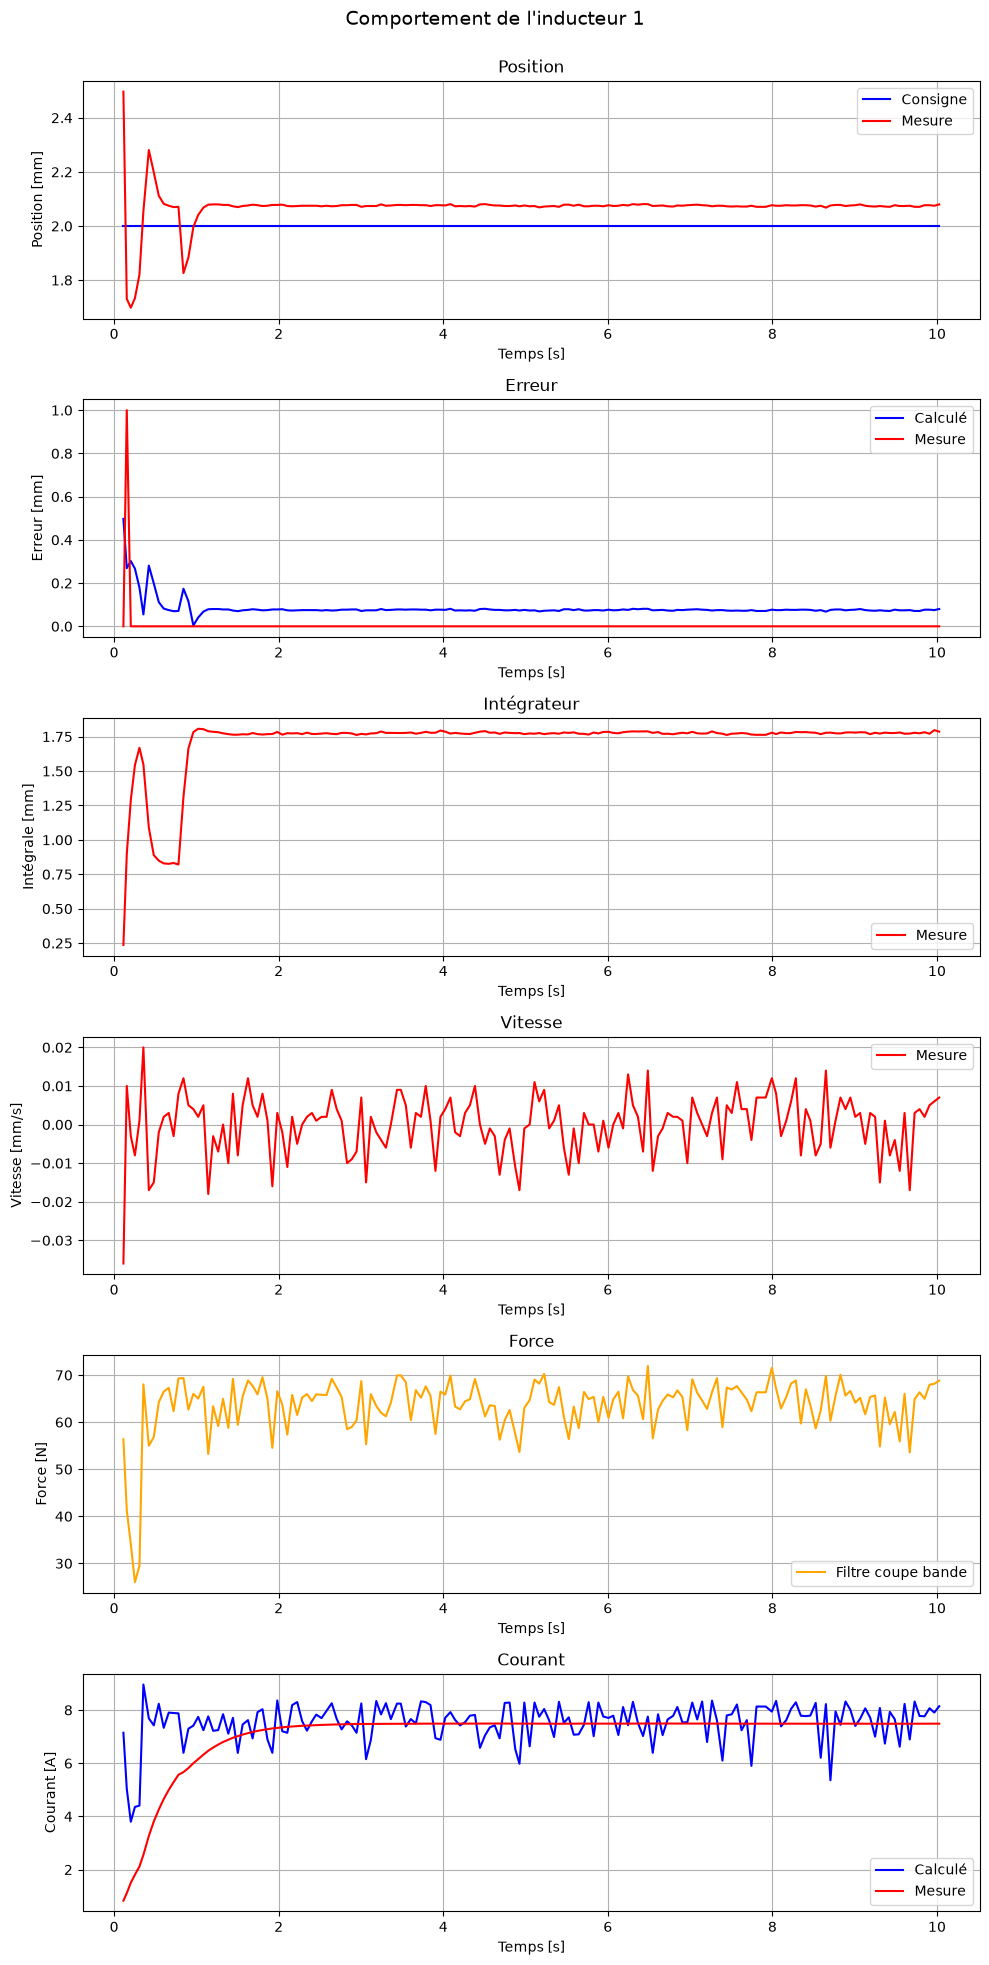
\includegraphics[width=0.8\linewidth]{assets/content/08-MesureProgPrinc/MesRegPos1.png}
    \caption{Évolution de la régulation de position pour l'inducteur 1}
    \label{fig:RegPosInd1}
\end{figure}

\begin{figure}[H]
    \centering
    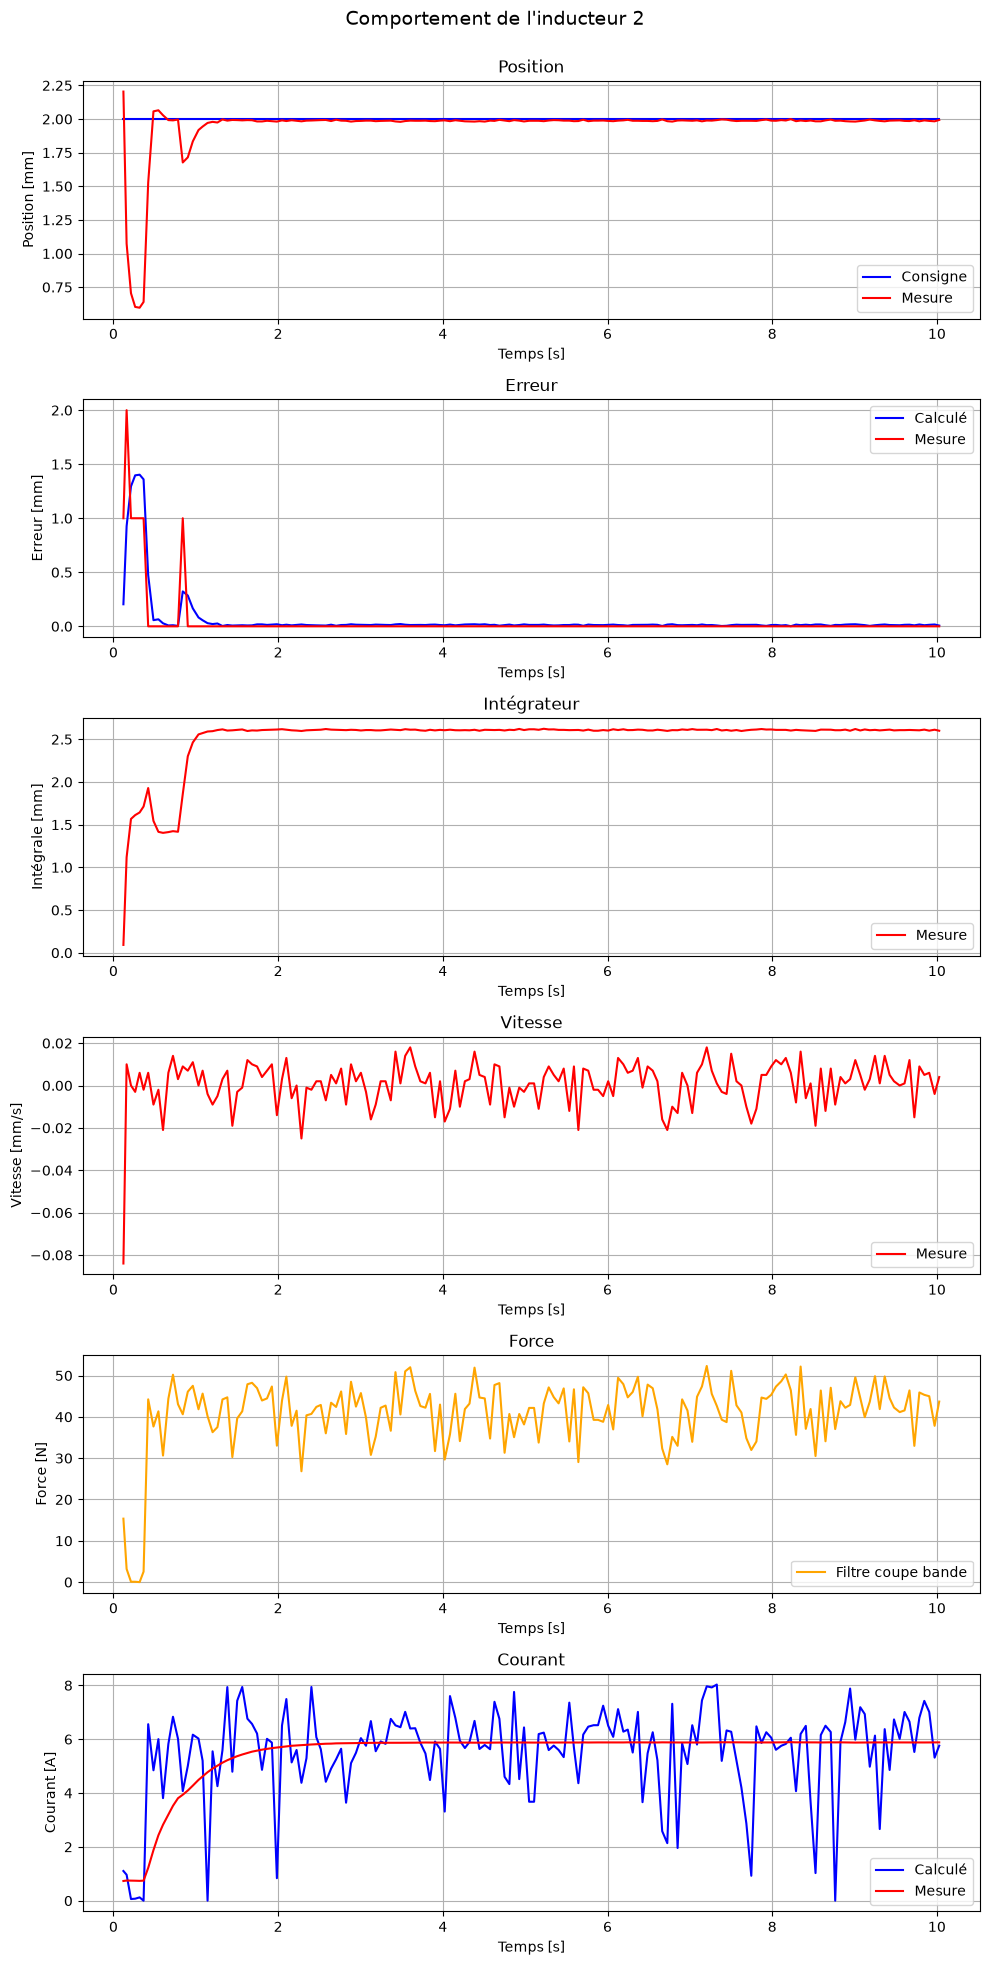
\includegraphics[width=0.8\linewidth]{assets/content/08-MesureProgPrinc/MesRegPos2.png}
    \caption{Évolution de la régulation de position pour l'inducteur 2}
    \label{fig:RegPosInd2}
\end{figure}

\begin{figure}[H]
    \centering
    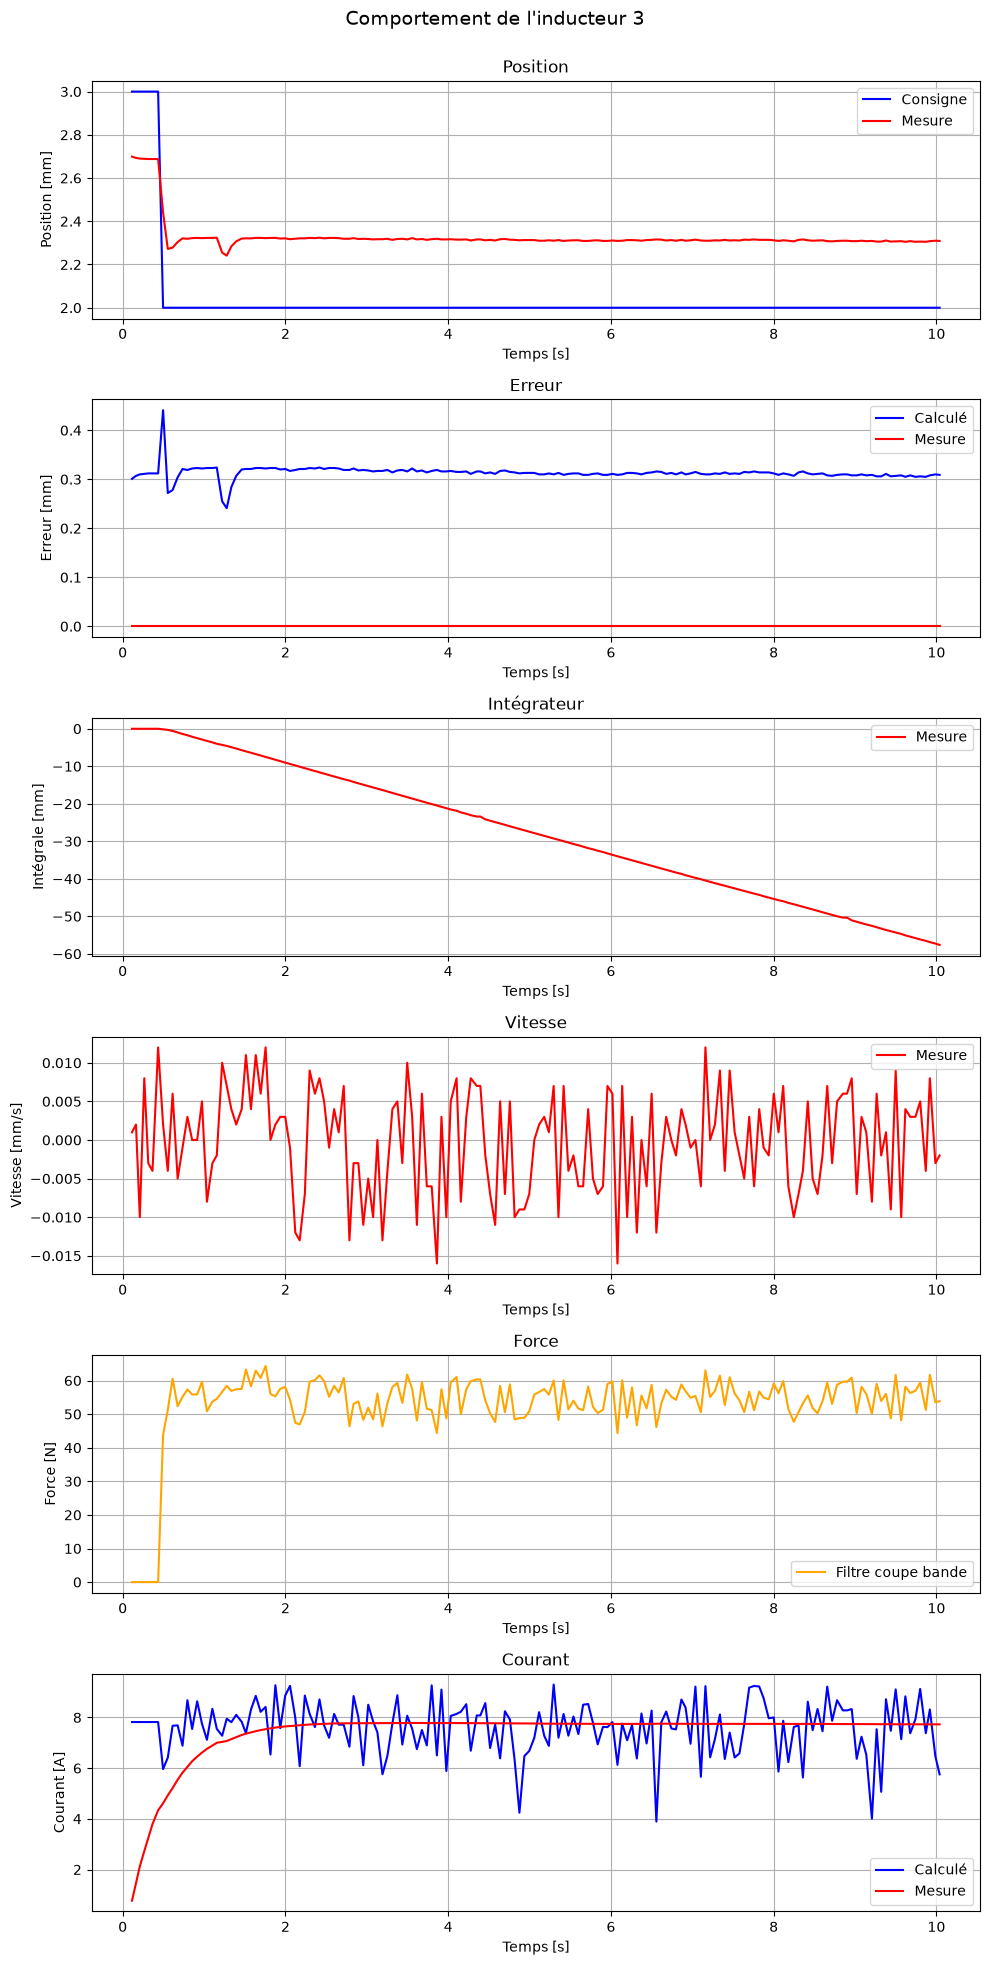
\includegraphics[width=0.8\linewidth]{assets/content/08-MesureProgPrinc/MesRegPos3.png}
    \caption{Évolution de la régulation de position pour l'inducteur 3}
    \label{fig:RegPosInd3}
\end{figure}

\begin{figure}[H]
    \centering
    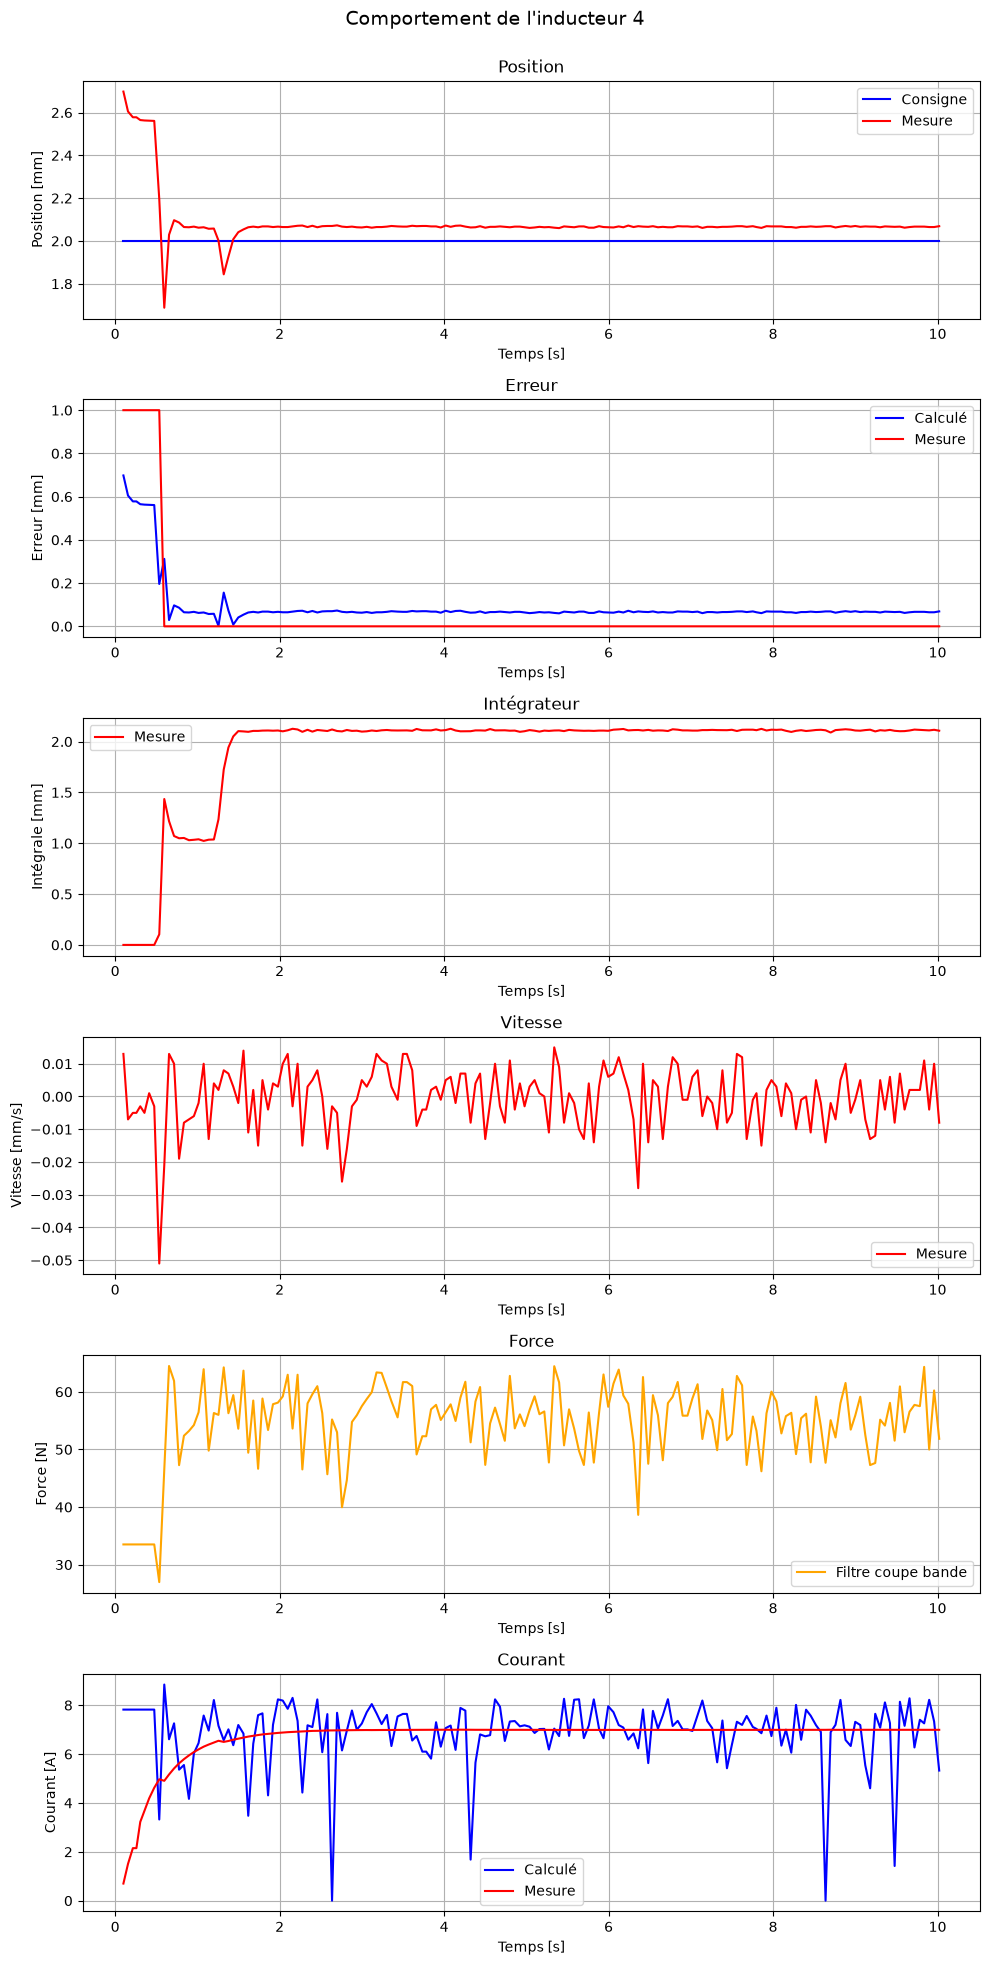
\includegraphics[width=0.8\linewidth]{assets/content/08-MesureProgPrinc/MesRegPos4.png}
    \caption{Évolution de la régulation de position pour l'inducteur 4}
    \label{fig:RegPosInd4}
\end{figure}

En se concentrant uniquement sur les consignes de force, la \autoref{fig:ForceInd} représente les différentes valeurs supposées être présentes dans le code :

\begin{figure}[H]
    \centering
    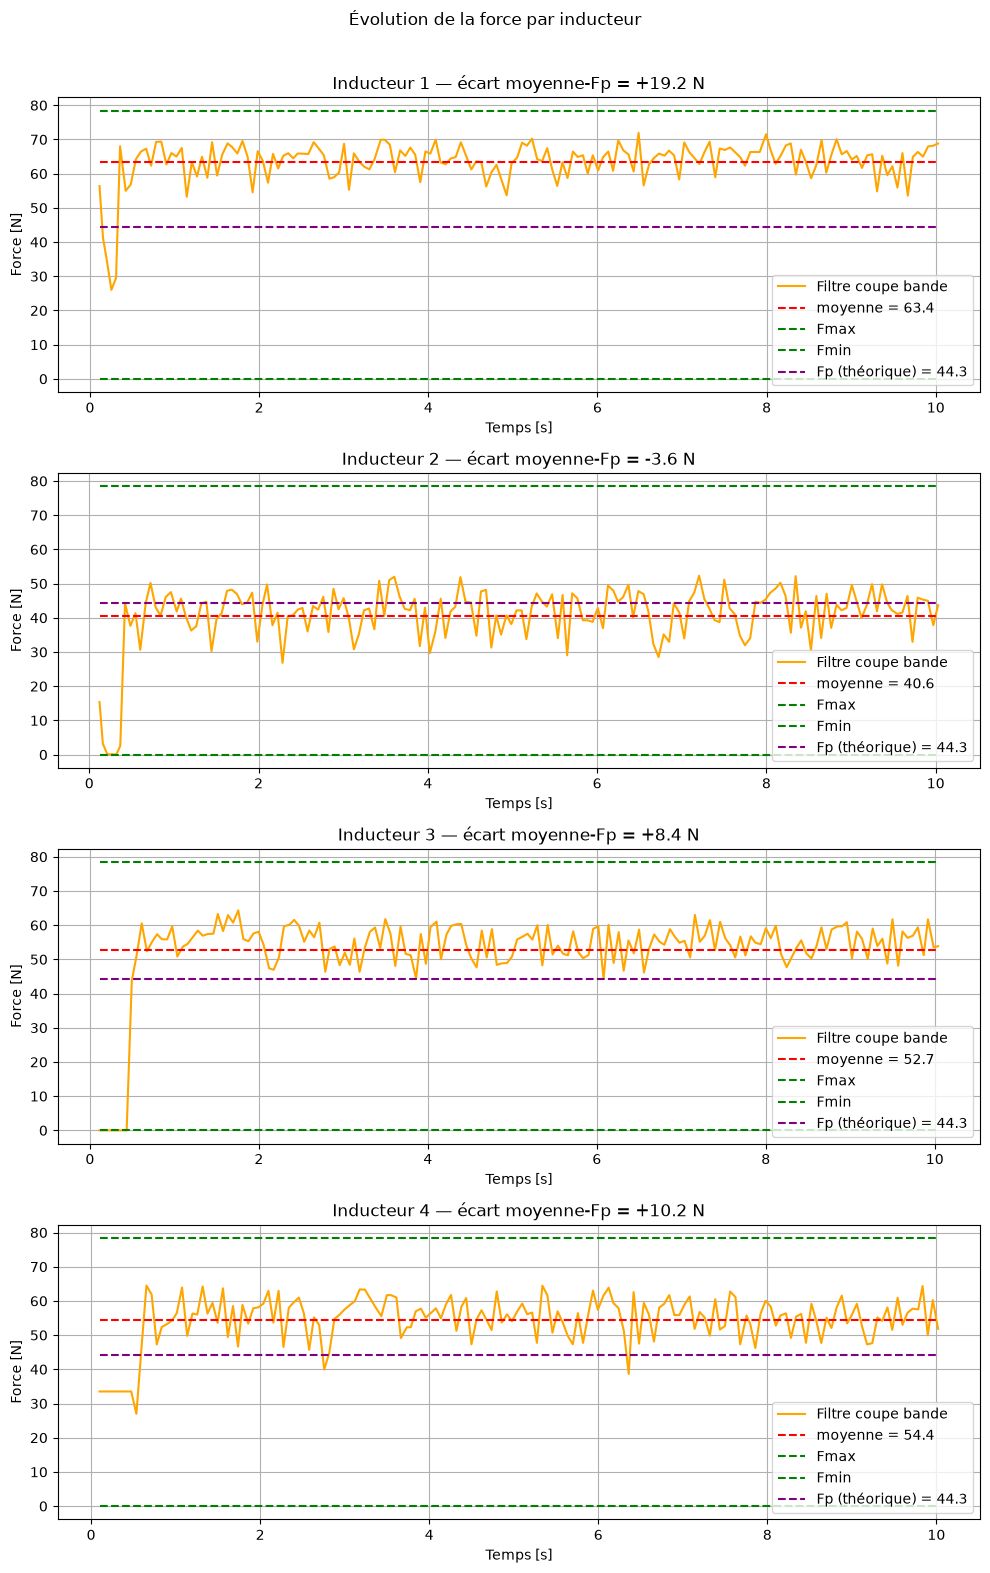
\includegraphics[width=0.85\linewidth]{assets/content/08-MesureProgPrinc/AnalyseForce.png}
    \caption{Évolution de la consigne de force par inducteur}
    \label{fig:ForceInd}
\end{figure}

Il est dès lors possible de calculer les écarts présententre la valeur théorique supposé et la valeur récupérer dans le code :

\begin{table}[H]
    \centering
    \begin{tabular}{l cccc}
        \toprule
        \textbf{Inducteur} & \textbf{Moyenne [N]} & \textbf{$F_p$ théorique [N]} & \textbf{Écart [N]} & \textbf{Écart [\%]} \\
        \midrule
        Inducteur 1        & 63.44                & 44.27                        & 19.17              & 43.29               \\
        Inducteur 2        & 40.63                & 44.27                        & -3.64              & -8.23               \\
        Inducteur 3        & 52.68                & 44.27                        & 8.41               & 18.99               \\
        Inducteur 4        & 54.43                & 44.27                        & 10.16              & 22.95               \\
        \bottomrule
    \end{tabular}
    \caption{Comparaison des forces moyennes et théoriques par inducteur}
    \label{tab:forces_inducteurs}
\end{table}

\subsection{Analyse des résultats}
En étudiant les différents résultats, certains points sont intéressants à retenir.

Tout d'abord, il est observable que pour l'inducteur 1, le résultat de l'erreur est régulièrement erroné. Celle-ci est annoncée à 0, mais en réalisant le même calcul que celui du code (soit la simple soustraction entre la mesure et la consigne), la trace bleue indique la valeur que devrait réellement posséder l'erreur. Cela peut toutefois s'expliquer par un manque de résolution lors de l'envoi des données. En effet, la position a été multipliée par mille après coup afin d'être affichée en millimètres et non en mètres. Ce comportement n'est cependant pas omniprésent, les autres inducteurs semblant indiquer des valeurs plus justes. Il est également probable que la mesure de l'inducteur 1 comportait une légère erreur à l'envoi.

Le second point à traiter est le résultat de la consigne de force. En analysant les résultat présent dans le \autoref{tab:forces_inducteurs}, il est possible de s'apercevoir que celle-ci ne se situe pas autour de la valeur théorique liée à la pesanteur. En effet, lorsque la maquette est en maintien, la force électromagnétique devrait être équivalente à la force de pesanteur, soit $F_{el} = 4.513\cdot9.81 = 44.3$~N. Or, cette valeur est régulièrement dépassée, ou au contraire non atteinte. L'écart entre la valeur théorique et la moyenne mesurée est présenté dans le \autoref{tab:forces_inducteurs} :

Une première explication à ce phénomène est que l'inductance réelle ne correspond pas à celle calculée, mais présente une valeur plus élevée. Cette hypothèse est vérifiée dans le chapitre suivant.

Une seconde explication serait due à une torsion du système entre les inducteurs : l'un s'appuyant sur l'autre, il nécessite alors une force bien plus importante que prévu pour atteindre la consigne de position désirée.

\section{Conclusion}
Les mesures ont permis de clarifier plusieurs points et de statuer sur une partie des hypothèses formulées dans la \autoref{sec:Hypothese}.

Tout d'abord, l'hypothèse selon laquelle la communication UART perturbe l'interruption principale est infirmée : aucun effet n'a été observé. L'hypothèse du non-respect des contraintes temporelles est également infirmée, les temps d'exécution mesurés laissant une marge importante par rapport à la période de 40~$\mu$s. Il aurait cependant été préférable de compléter l'analyse en réglant le déclenchement de l'oscilloscope sur une durée d'impulsion minimale, afin de vérifier si l'interruption est réellement arrêtée plus tôt que prévu. Cette piste n'a pas été explorée davantage.

La seconde mesure a mis en évidence des comportements étranges concernant la régulation de position : une erreur transmise incohérente sur l'inducteur 1 et, surtout, des consignes de force s'écartant notablement de la valeur théorique de pesanteur. L'hypothèse d'un calcul d'erreur incorrect dans la boucle de position ne peut donc être ni confirmée ni infirmée à ce stade. Les chapitres suivants poursuivent les recherches nécessaires pour clarifier le phénomène de la force.